\section{First model}

The Jupyter Notebook concerning this chapter can be viewed via \url{https://srp.klawr.de/\#5}.

\subsection{Structure}
The project structure is an important part of efficiently testing models and evaluation them against another to determine the best performing one.
\name{deepmech} is structured using a modified version of the Cookiecutter Data Science \cite{drivendata2019} structure. It can be inspected at \url{klawr.github.io/deepmech}.

% root
The root folder contains files like the License of the whole project.
The project is licensed under the MIT license providing any human to modify, distribute or use it for private and commercial use, but omitting any liability or warranty from myself.
In the root folder another file requirements.txt is found, which is part of the installation process allowing to replicate all code discussed in this project.

% data
The Cookiecutter Data Science structure allows for a clear distribution of data in raw (which is never to be touched), intermediate (which is the raw data but modified, augmented or altered in some way) and processed data (which is to be fed into the model via a training algorithm).

% logs
Logs are filled during training using \name{Tensorboard}\footnote{Tensorboard is \name{Tensorflow}'s visualization toolkit. Visualizations generated using \name{Tensorboard} are shown later.}. Logs are differentiated using a timestamp of the respective training run.

% TODO models folder...

% reports
A folder containing all reports used in the project are found in the respective directory, including this very article.
In the notebook folder in reports for this project (abbreviated as \name{srp}) one can find the code used to determine the best model.
Models are trained using \name{Jupyter Notebooks} \cite{Jupyter2019}.
Jupyter Notebooks an interactive editor to develop Python code, which provide an easy way to write and test code efficiently.
All notebooks with respective code are to be found in the \name{notebooks} directory in the root of this project\footnote{\url{https://srp.klawr.de/\#6}}.
% src
\name{src} contains all code (except demos used in the reports) used in developing and training the models. They range from scripts which create adequate environments to train models, to data augmentation.

\subsection{Loading data}
Before the training of the model can start data has to be loaded.
As mentioned the data is saved in the \name{raw} directory of the \name{data} directory in this project.
It is good practice to never work with the raw data directly, therefore the beginning of each training session contains a preparation phase, where the raw data is to be copied to the \name{processed} data directory (maybe with augmentations or alterations in intermediate steps).

That being said, every training of a model in this project starts using the following code:

\begin{lstlisting}
from os.path import join

raw = join('data', 'raw')
interim = join('data', 'interim')
processed = join('data', 'processed')
    
from src.training_env import reset_and_populate
    
reset_and_populate(raw, processed, [400, 0, 100])
\end{lstlisting}

For the first model the raw data itself suffices; therefore it is just copied into the processed data directory using a predefined function from \code{training\_env.py}.
\code{reset\_and\_populate}'s third parameter is an array containing three numbers describing the distribution of training, validation and test data.
For this very example, the validation data is omitted, because no adjustments on the hyper parameters are made.

\begin{lstlisting}
from tensorflow.keras.preprocessing.image import ImageDataGenerator

def create_generator(data_dir, batch_size):
    datagen = ImageDataGenerator(rescale=1./255)
    full_path = join(processed, data_dir)
    return datagen.flow_from_directory(
        full_path,
        target_size=(32, 32),
        batch_size=batch_size,
        class_mode='binary')

train_generator = create_generator('train', 20)
test_generator = create_generator('test', 10)
\end{lstlisting}

After the respective directories are populated, \code{ImageDataGenerator}\footnote{\url{https://keras.io/preprocessing/image/}} is used to allow the model to load the data later in the training process.
The generators also defines the size of the image loaded, which is set to be 32 pixels wide and 32 pixels high (in contrast to the original image size of 512x512) and a batch size\footnote{The batch size is the number of images used between each backpropagation cycle.
If the batch size matches the dataset size it is called batch gradient descent, if the batch size is one it is called stochastic gradient descent.
Everything in between is called mini-batch gradient descent.} of 20 is set.
The \code{class\_mode} is set to \code{'binary'}, since the input consists of 1D numpy arrays.
These generators also detect the structure of the raw data (distributed in repective directories using their label as directory name) and thereby assigns labels to them.

\subsection{Creation of the model}

\begin{lstlisting}[label={lst:first_model}]
from tensorflow.keras import layers
from tensorflow.keras import models

model = models.Sequential()
model.add(layers.Flatten(input_shape=(32, 32, 3)))
model.add(layers.Dense(32,'relu'))
model.add(layers.Dense(32,'relu'))
model.add(layers.Dense(3, 'softmax'))

model.summary()
\end{lstlisting}

All models used in this project are sequential models.
Sequential models propagate the result of each layer on to the next in a one-way fashion.

\name{Keras} requires the first layer to have an \code{input\_shape}.
The input shape of the first model has to match the actual size of the input data.
All other layers are able to deduce the shape of the previous layer, so no further definitions are needed.

Layers can be added by using a provided \code{add} function which accepts layers as parameters which are subsequently added to the model.

The first layer is just a representation of the input image as pixel values.
They are flattened, so the two dimensional image gets projected into a one dimensional array.

Two layers are added, both being dense layers with 32 nodes each.
Dense layers are defined by connecting all nodes of the previous layer via weights and biases to the nodes on their own layer and behaving like "traditional" layers used in this project.
The two hidden layers are activated using the \name{'relu'} activation, as suggested in \cite[p.168]{Goodfellow2017}.

The last layer has three nodes in respect to three classes the data can be assigned to.
The \name{'softmax'} activation is used, which adjusts the values of the layer to add up to the value one.
Therefore the value of the node can be seen as a measure of the confidence of the evaluation of the model for a specific input.
Naturally the node with the highest value is representing the assumed correct result.

A summary of the model is given as:
\begin{lstlisting}
Model: "sequential"
_________________________________________________________________
Layer (type)                 Output Shape              Param #   
=================================================================
flatten (Flatten)            (None, 3072)              0         
_________________________________________________________________
dense (Dense)                (None, 32)                98336     
_________________________________________________________________
dense_1 (Dense)              (None, 32)                1056      
_________________________________________________________________
dense_2 (Dense)              (None, 3)                 99        
=================================================================
Total params: 99,491
Trainable params: 99,491
Non-trainable params: 0
_________________________________________________________________
\end{lstlisting}

Herein we can see, that the model has 99491 parameters in $\theta$ which are to be adjusted. This number is the sum of parameters given by the 3 individual layers of the model.
The first layer has the flattened 3072 ($32 \times 32 \times 3$) nodes.
The second layer multiplies this number (+1 for bias) by $32$ and therefore has additional 98336 nodes.
The third layer is the product of $32 + 1$ nodes in the second layer and $32$ nodes in the third, providing us with 1056 parameters to adjust.
The last layer has again $(32 + 1) \times 3$ layers.

\subsection{Optimizer}

To train our model an optimizer has to be defined.
We will start with a \code{SGD} optimizer, which is short for \name{Stochastic Gradient Descent}. Stochastic Gradient Descent is already mentioned in chapter~\ref{ch:simple_linear_example}, where it was implemented in a very rudimentary way. In the actual training of the model the Keras implementation is used.
Keras implementation of SGD is somewhat different than the general definition, because it does not inherently take a batch size of one, but the batch sizes defined in the respective generator, thus letting the user decide if full batch, mini batch or stochastic gradient descent is used (which is 20 in this case).

\begin{lstlisting}
optimizer = SGD(lr=0.01, momentum=0.9, nesterov=True)
\end{lstlisting}

The \code{SGD} function takes three parameters: The learning rate \code{lr}, \code{momentum} and \code{nesterov}.
These values are again hyper-parameters which have to be determined before training.

\subsubsection{Learning rate}
% TODO put some citations in here...

The learning rate is one of the most influential hyper parameters and arguably the most profound, as it is being used in almost every optimizer.
It is a scalar value which determines the step size of the steps taken. Recall that the update function of the parameter $\theta$ is:
\begin{equation}
    \theta_{i+1} := \theta_i - \eta \varDelta \tag{\ref{eq:backprop_update} revisited}
\end{equation}.
Where $\eta$ is the value of the learning rate.

If the learning rate is set to a value too small, the loss function takes a lot of iterations to converge to a sufficiently small value.
On the other hand a learning rate set to a high value may fail to converge at all.

\begin{figure}
    \centering
    \begin{subfigure}[b]{0.3\textwidth}
        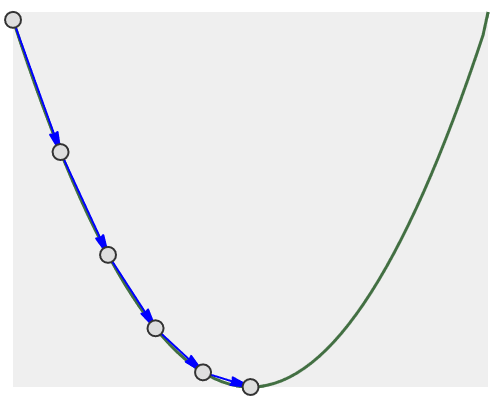
\includegraphics[width=\textwidth]{images/lr_ok.png}
        \caption{Learning rate just right}
        \label{fig:lr_ok}
    \end{subfigure}
    \begin{subfigure}[b]{0.3\textwidth}
        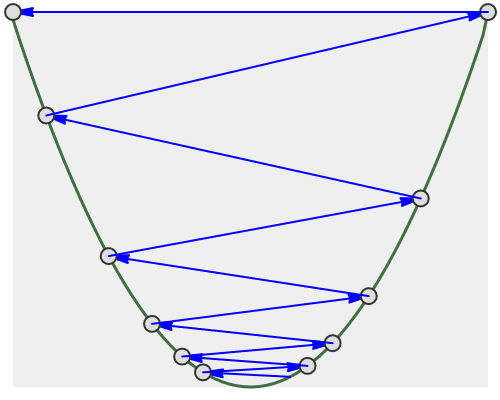
\includegraphics[width=\textwidth]{images/lr_too_high.png}
        \caption{Learning rate too high}
        \label{fig:lr_too_high}
    \end{subfigure}
    \begin{subfigure}[b]{0.3\textwidth}
        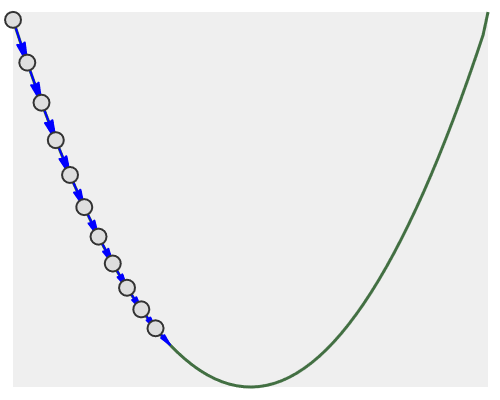
\includegraphics[width=\textwidth]{images/lr_too_low.png}
        \caption{Learning rate too small}
        \label{fig:lr_too-low}
    \end{subfigure}
    \caption{If the learning rate is just right, the value of the loss function converges to a local optimum in an acceptable number of steps.
    If it is too high it diverges.
    If the learning rate is too low, the values converge but they take too many steps to do so.
    Please note that these images represent the parameter space in a very simplified way, as the presented function it is fully convex and only two dimensional.}
    \label{fig:learning_rate}
\end{figure}

\subsubsection{Momentum}

Introduced 1964 by Polyak \cite{Polyak1964} momentum is used to keep the gradient consistent over several steps.
Momentum takes its name as an analogy to the physical effect according to Newton's second law of motion.
The direction of the correction through the gradient should be consistent over several steps and it would be peculiar if the direction makes sudden shifts throughout training.
This is useful if the data is noisy or some of the training examples are falsy.
Hence another parameter $\nu$ is introduced to equation~\eqref{eq:backprop_update}:

\begin{equation}
    \begin{split}
        \nu_{i} &:= \alpha \nu_{i-1} - \eta \varDelta \\
        \theta_{i+1} &:= \theta_i + \nu_i
    \end{split}
    \label{eq:momentum}
\end{equation}

Whereas $\alpha$ is another parameter which can be set to regulate the influence of $\eta$ on the parameters of the next iteration.
So if one training example would change the "direction" of the next step with a high deviation from the median of the last few steps the impact would be reduced and may improve the rate of convergence.

In 2013 Sutskever, Martens, Dahl and Hinton \cite{Sutskever2013} introduced another variant of momentum which was inspired by Nesterov's Accelerated Gradient \cite{Nesterov1983}.
This variant updates the previous discussed equation to change the parameter used to calculate $\varDelta$ using $\nu$.
Please note that $\varDelta$ in equation~\eqref{eq:momentum} and ~\eqref{eq:backprop_update} is itself a function of the parameter $\theta$ (see equation~\eqref{eq:hidden_error}).

\begin{equation}
    \begin{split}
    \nu_i & := \alpha \nu_i - \eta \varDelta(\theta_i + \alpha \nu_i) \\
    \theta_{i+1} & := \theta_i + \nu_i
    \end{split}
    \label{eq:nesterov}
\end{equation}

The idea of momentum being that the directional vector points in the right direction, using Nesterov Accelerated Gradient is likely to be more accurate by starting to measure the next error slightly shifted into the respective direction \cite[p.353]{Geron2019} \cite[p.291]{Goodfellow2017}.

\subsubsection{Actual training}

After the optimizer is defined, the model is compiled by issuing the models compile function.

\begin{lstlisting}
model.compile(
    loss='sparse_categorical_crossentropy', 
    optimizer=optimizer,
    metrics=['acc'])
\end{lstlisting}

\code{sparse\_categorical\_crossentropy} is used as loss function as advised for multi class categorization problems labeled by integers \cite[p.84]{Chollet2017}.
It measures the distance of two probability distributions, which are given by the last layer of the model, given by a \code{softmax} activation and the labeled data.
SoftMax activation is used to normalize the output by dividing each value by the sum of all values in the respective layer.
This is useful because the labeled data assigns the value one to the correct node and zero to all others, making them numerically comparable and thereby possible to minimize the loss for a sensible result.

The actual training is done by a \code{fit} function in the model.
The training data is provided as generators; the function in this case is \code{fit\_generator}.
Therefore by issuing the following function the training is performed:
% TODO python and remove generator
\begin{lstlisting}
history = model.fit_generator(
    train_generator,
    steps_per_epoch=20,
    epochs=20,
    callbacks=callbacks)
\end{lstlisting}

Herein it is defined that 20 images are fed into the model each iteration, which is repeated for 20 epochs.
An epoch being one run-through, so the optimizer updates the parameters 20 times.

\subsubsection{Results}
\begin{figure}
    \centering
    \begin{subfigure}[b]{0.4\textwidth}
        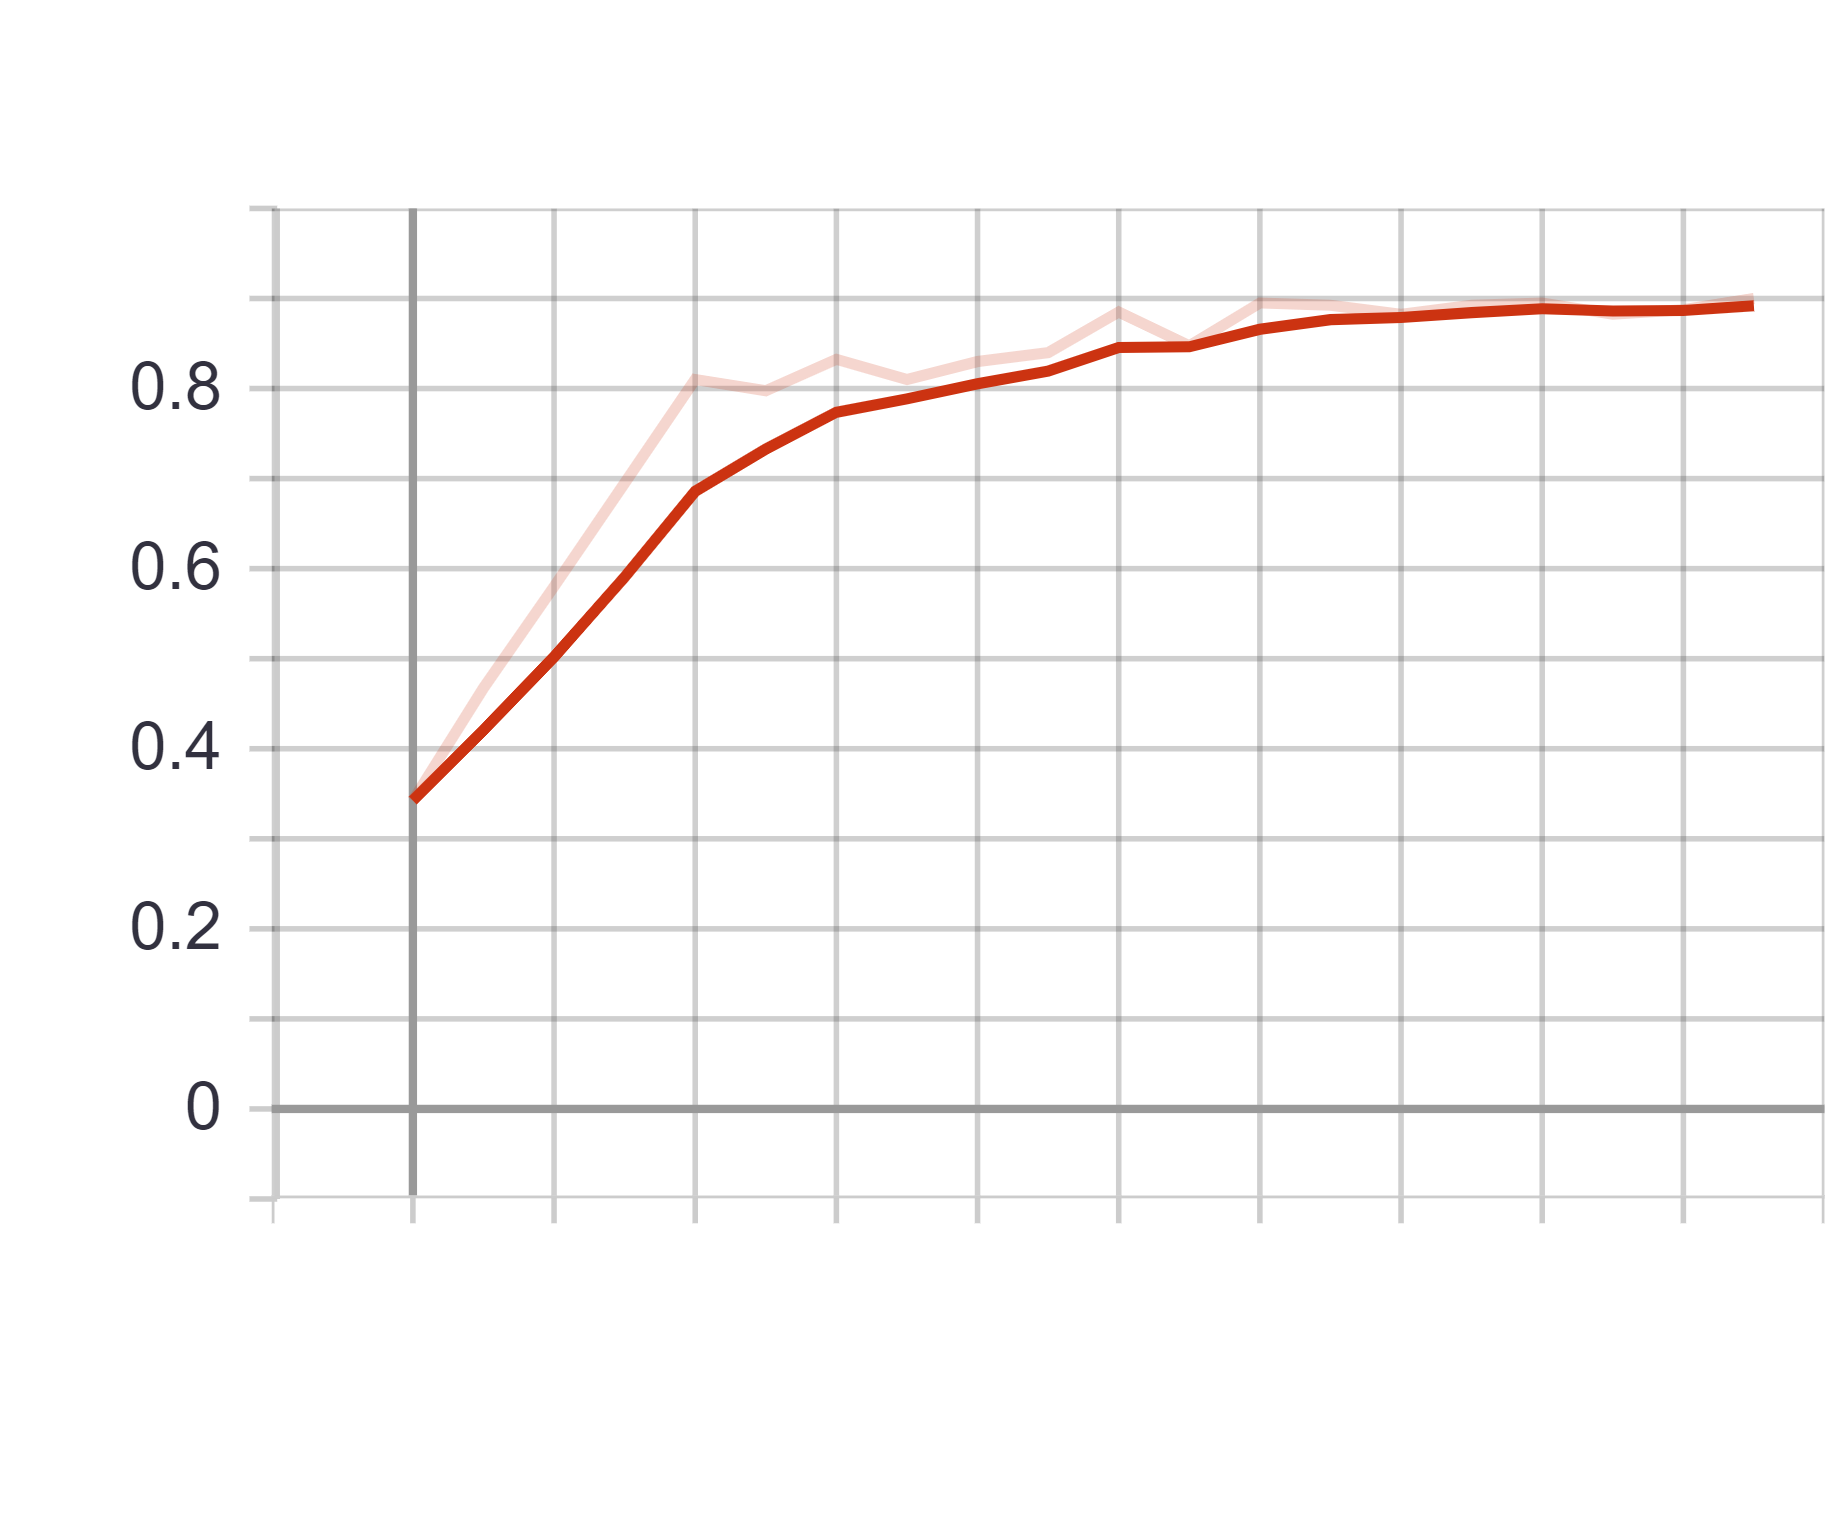
\includegraphics[width=\textwidth]{images/first_model_acc.png}
        \caption{Accuracy}
        \label{fig:first_model_acc}
    \end{subfigure}
    \begin{subfigure}[b]{0.4\textwidth}
        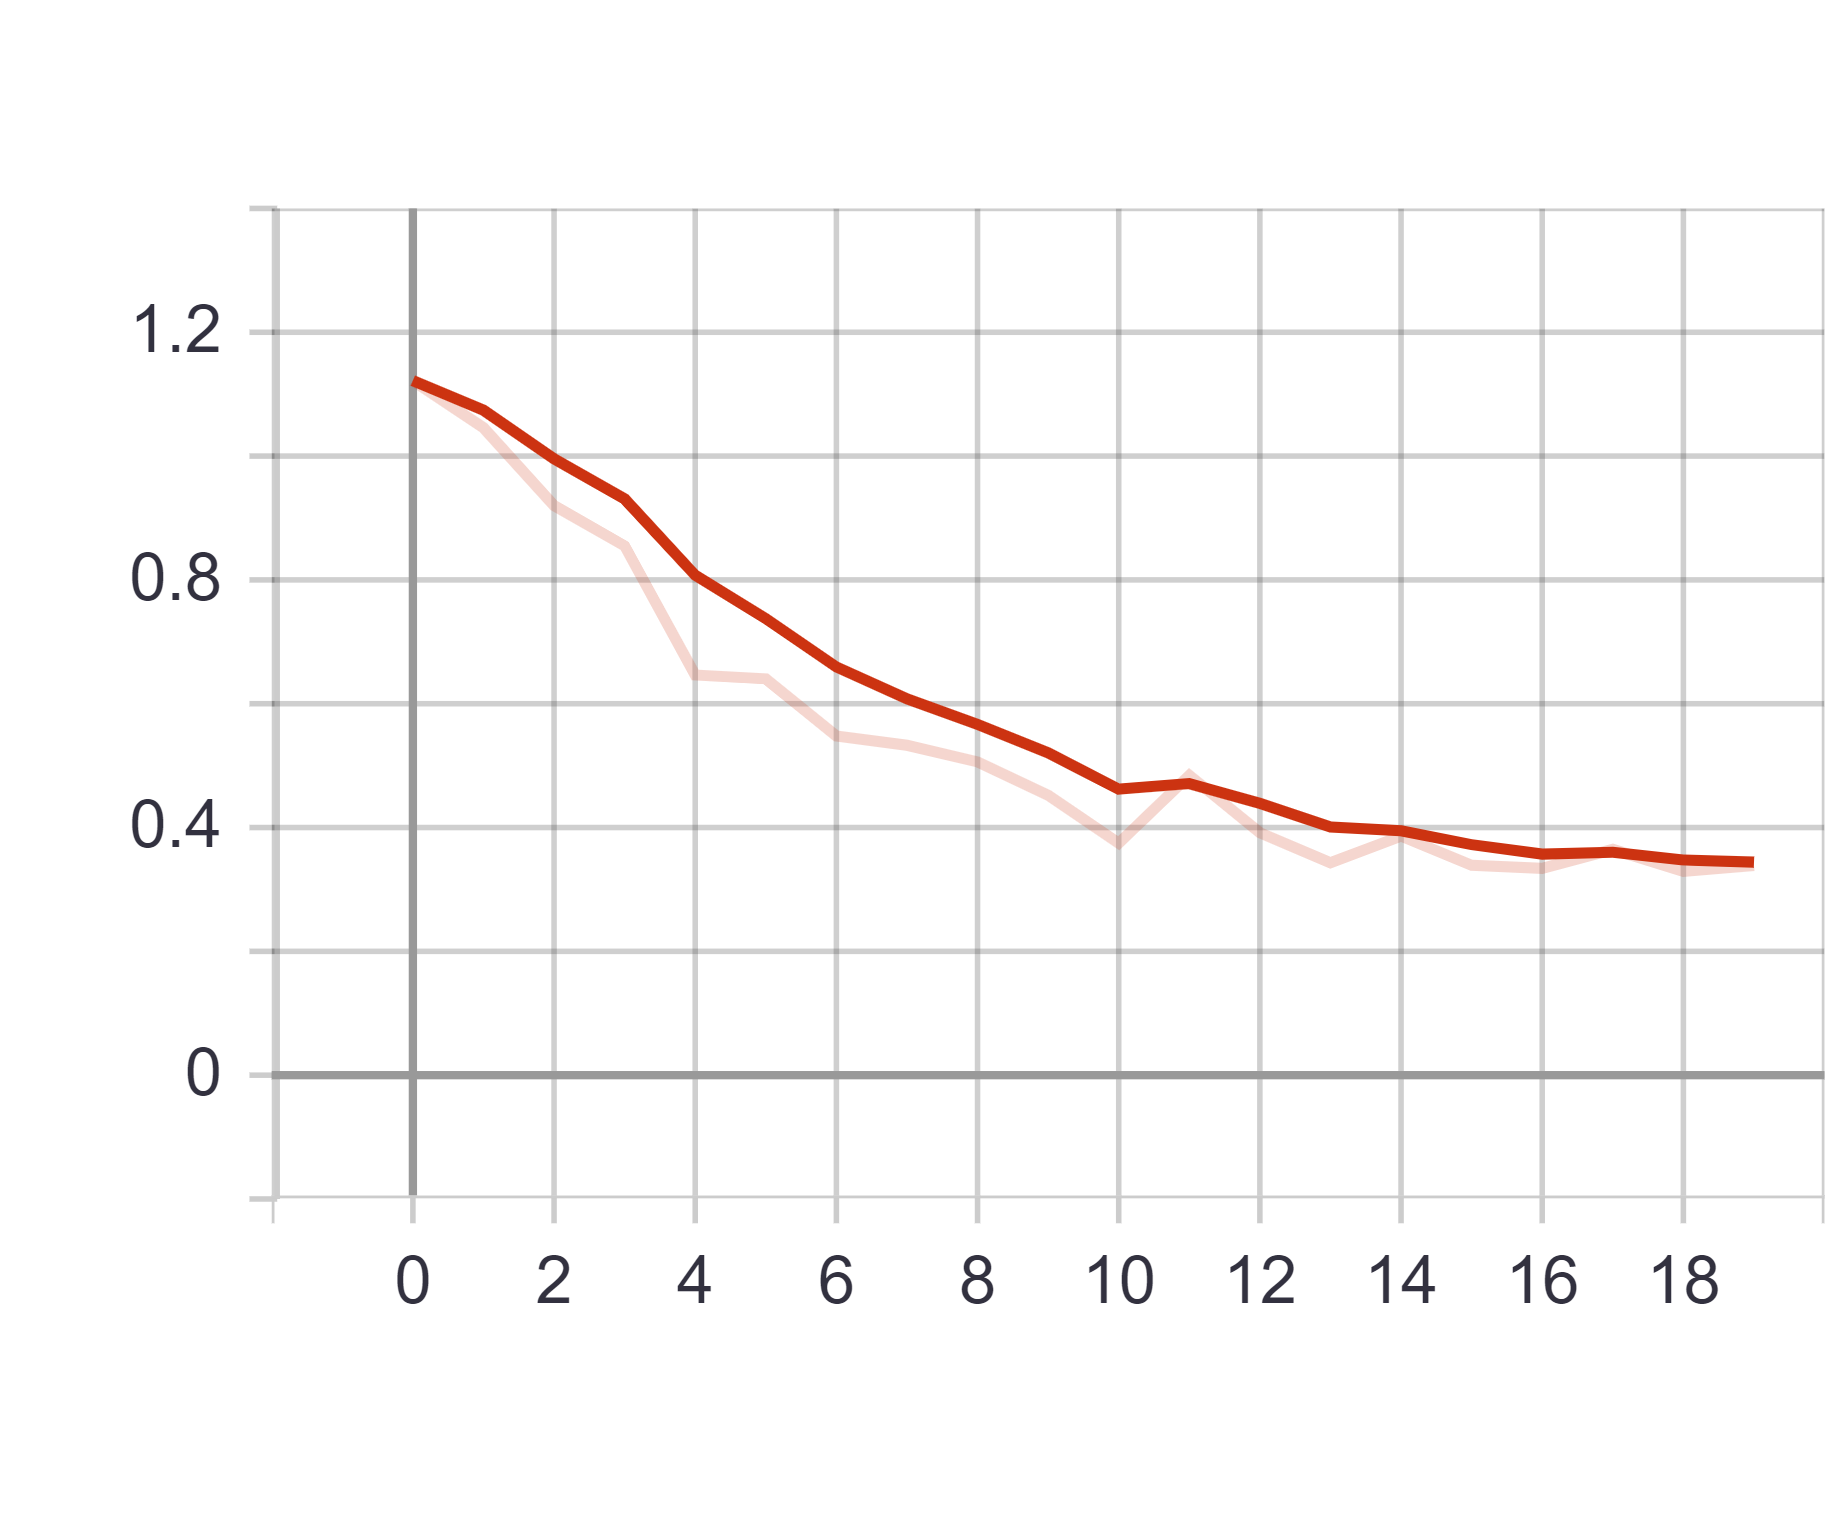
\includegraphics[width=\textwidth]{images/first_model_loss.png}
        \caption{Loss}
        \label{fig:first_model_loss}
    \end{subfigure}
    \caption{The callbacks of the training algorithm provide logs which can be used by TensorBoard to provide useful graphs to evaluate the model. The vertical axis represents the value on the respective epoch (shown on the horizontal axis).}
    \label{fig:first_model_graphs}
\end{figure}

As it is expected the model begins with an accuracy of approximately 33\% by trying to classify training data into three classes.
As the data suggests, the model is quickly learning some relations between input data and the respective label, as it already has an accuracy of almost 70\% after only four epochs.

\begin{lstlisting}
Epoch 1/20
20/20 [=====...=====] - 2s 79ms/step - loss: 1.1220 - acc: 0.3425
Epoch 2/20
20/20 [=====...=====] - 1s 55ms/step - loss: 1.0457 - acc: 0.4675
Epoch 3/20
20/20 [=====...=====] - 1s 55ms/step - loss: 0.9199 - acc: 0.5800
Epoch 4/20
20/20 [=====...=====] - 1s 46ms/step - loss: 0.8548 - acc: 0.6950
...
Epoch 17/20
20/20 [=====...=====] - 1s 45ms/step - loss: 0.3340 - acc: 0.8950
Epoch 18/20
20/20 [=====...=====] - 1s 48ms/step - loss: 0.3648 - acc: 0.8825
Epoch 19/20
20/20 [=====...=====] - 1s 52ms/step - loss: 0.3291 - acc: 0.8875
Epoch 20/20
20/20 [=====...=====] - 1s 47ms/step - loss: 0.3388 - acc: 0.9000
\end{lstlisting}

After 20 epochs the model has an accuracy of roughly 90\%, which is already a very good start for a first model with non optimized hyper-parameters.
The important thing for a working model is how well the model classifies data which it has never seen before.
To check this a second generator is created: the \code{test\_generator} which is used to evaluate the model.
By issuing \code{model.evaluate\_generator(test\_generator)} we get \code{[0.6071663084129493, 0.7866667]}, which indicates that the loss is at \code{0.60} in contrast to \code{0.33} on the training data and has and accuracy of 78\% on data is has never seen before.

This result is quite remarkable, but obviously the model performs worse on new data, therefore indicating it is overfitting on the training data.
Notwithstanding the above the result shows that by adjusting the hyper-parameters the result may be increased to a satisfying result.

After the model is trained it is saved into \name{models/symbol\_classifier/first\_model.h5} and may be loaded into Keras for further inspection.